\documentclass{article}

\usepackage{graphicx}
\usepackage{tikz}
\usepackage{tikzsymbols}
\usetikzlibrary{calc,patterns,shapes.geometric}
\pagestyle{empty}
\usepackage[margin=0pt]{geometry}
\geometry{papersize={14in,12in}}

\def\centerarc[#1](#2)(#3:#4:#5){\draw[#1] ($(#2)+({#5*cos(#3)},{#5*sin(#3)})$) arc (#3:#4:#5);}

\begin{document}
	\begin{figure}
		\centering
		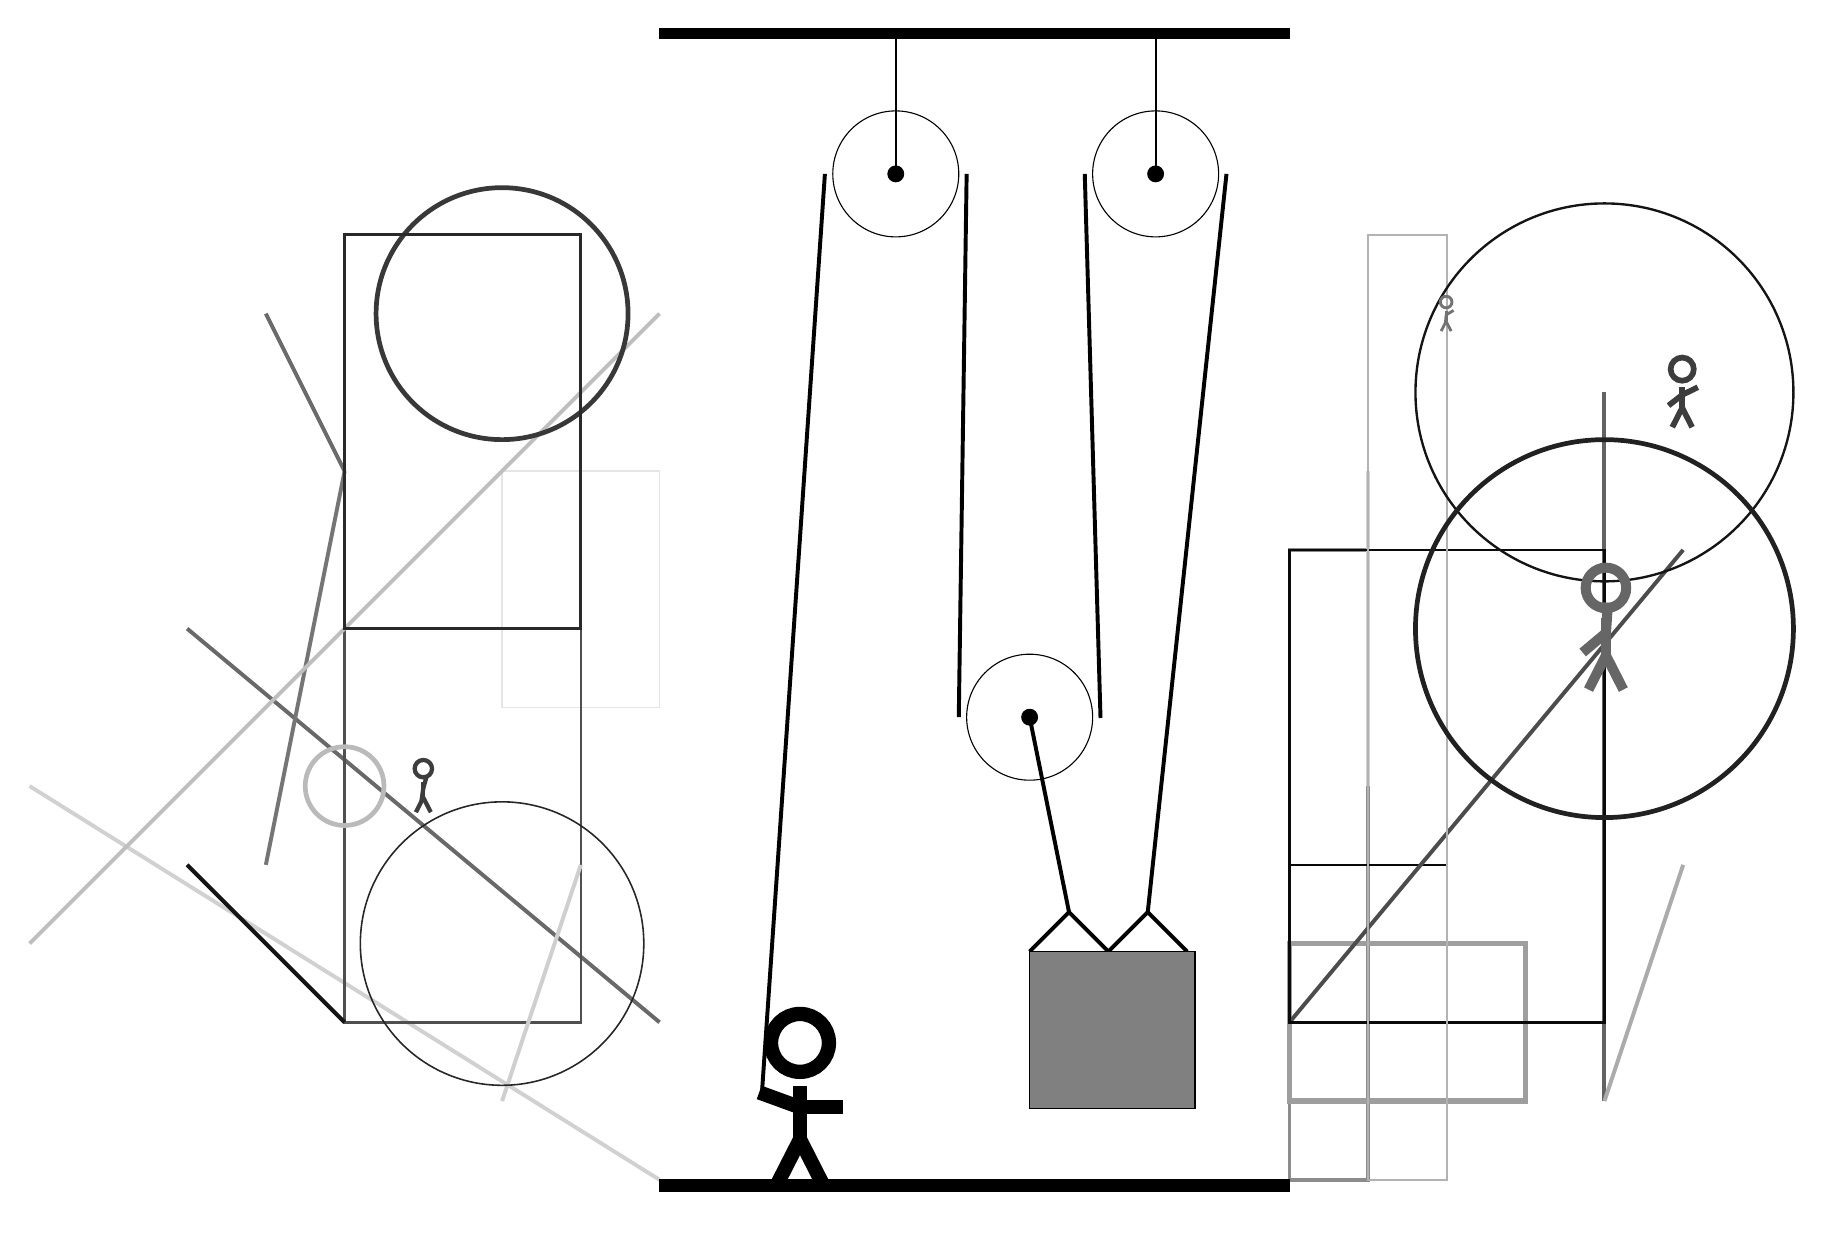
\begin{tikzpicture}
			%%%%% START %%%%%
			
			\draw[fill=black] (-2, 11.5) rectangle (6, 11.625);
			
			\draw[line width=0.5mm, color=black!18](-2, -3) -- (-10, 2);
			
			\draw[line width=0.5mm, color=black!45] (6, 5) rectangle (7, -3);
			\draw[line width=0.5mm, color=black!59](-2, -1) -- (-8, 4);
			\node[line width=0.4mm, color=black!76] at (11, 7) {\Strichmaxerl[4][38][26]};
			\draw[line width=0.2mm, color=black!10] (-2, 6) rectangle (-4, 3);
			
			\draw[line width=0.2mm, color=black!22] (7, -3) rectangle (8, 0);
			\draw[line width=0.3mm, color=black!97] (8, -2) rectangle (6, 1);
			
			\draw[line width=0.3mm, color=black!69] (-3, 9) rectangle (-6, -1);
			\draw[line width=0.5mm, color=black!17] (7, 2) rectangle (7, 6);
			\draw[line width=0.5mm, color=black!61](10, 7) -- (10, -2);
			\draw[line width=0.5mm, color=black!58](-6, 6) -- (-7, 8);
			
			\draw[line width=0.7mm, color=black!38] (6, -2) rectangle (9, 0);
			\draw[line width=0.5mm, color=black!70](6, -1) -- (11, 5);
			\draw [line width=0.6mm, color=black!27](-6, 2) circle (0.5);
			\draw[line width=0.5mm, color=black!54](-6, 6) -- (-7, 1);
			\draw[line width=0.3mm, color=black!96] (6, -1) rectangle (10, 5);
			\draw[line width=0.5mm, color=black!25](-2, 8) -- (-10, 0);
			\draw[line width=0.2mm, color=black!30] (8, -3) rectangle (7, 9);
			\draw[line width=0.5mm, color=black!92](-6, -1) -- (-8, 1);
			\draw [line width=0.6mm, color=black!78](-4, 8) circle (1.6);
			\draw[line width=0.5mm, color=black!19](-4, -2) -- (-3, 1);
			
			\draw [line width=0.3mm, color=black!92](10, 7) circle (2.4);
			\node[line width=0.7mm, color=black!60] at (10, 4) {\Strichmaxerl[7][40][86]};
			\draw[line width=0.5mm, color=black!33](10, -2) -- (11, 1);
			\draw [line width=0.2mm, color=black!85](-4, 0) circle (1.8);
			
			\node[line width=0.7mm, color=black!55] at (8, 8) {\Strichmaxerl[2][85][31]};
			\draw[line width=0.4mm, color=black!84] (-3, 4) rectangle (-6, 9);
			\draw [line width=0.6mm, color=black!87](10, 4) circle (2.4);
			\node[line width=0.7mm, color=black!76] at (-5, 2) {\Strichmaxerl[3][82][74]};
			
			
			\draw (1, 9.775) circle (0.8);
			\draw[fill=black] (1, 9.775) circle (0.1);
			\draw[thick] (1, 9.775) -- (1, 11.5);
			
			\draw (4.3, 9.775) circle (0.8);
			\draw[fill=black] (4.3, 9.775) circle (0.1);
			\draw[thick] (4.3, 9.775) -- (4.3, 11.5);
			
			\draw (2.7, 2.875) circle (0.8);
			\draw[fill=black] (2.7, 2.875) circle (0.1);
			
			\draw[line width=0.5mm]  (2.7, -0.1) -- (3.2, 0.4) -- (3.7, -0.1) -- (4.2, 0.4) -- (4.7, -0.1);
			\draw[fill=black!50] (2.7, -0.1) rectangle (4.8, -2.1);
			
			\draw[line width=0.5mm](-0.7, -1.9) -- (0.1, 9.775);
			\centerarc[line width=0.5mm](1, 9.775)(0:180:0.9);
			\draw[line width=0.5mm](1.9, 9.775) -- (1.8, 2.875);
			\centerarc[line width=0.5mm](2.7, 2.875)(180:370:0.9);
			\draw[line width=0.5mm] (3.6, 2.865) -- (3.4, 9.775);
			\centerarc[line width=0.5mm](4.3, 9.775)(0:180:0.9);
			\draw[line width=0.5mm](4.2, 0.4) -- (5.2, 9.775);
			\draw[line width=0.5mm] (3.2, 0.4) -- (2.7, 2.875);
			
			\node at (-0.2, -2) {\Strichmaxerl[10][-20][0]};
			
			\draw[fill=black] (-2, -3) rectangle (6, -3.15);
			
			%%%%% END %%%%%
		\end{tikzpicture}
	\end{figure}	
\end{document}